%%%%%%%%%%%%%%%%%%%%%%%%%%%%%%%%%%%%%%%%%%%%%%%%%%%%%%%%%%%%%%%%%%%%%%%%%%%%%%%%
%%%%%%%%%%%%%%%%%%%%%%%%%%%%%%%%%%%%%%%%%%%%%%%%%%%%%%%%%%%%%%%%%%%%%%%%%%%%%%%%
%%% Template for AIMS Rwanda Assignments         %%%              %%%
%%% Author:   AIMS Rwanda tutors                             %%%   ###        %%%
%%% Email: tutors2017-18@aims.ac.rw                               %%%   ###        %%%
%%% Copyright: This template was designed to be used for    %%% #######      %%%
%%% the assignments at AIMS Rwanda during the academic year %%%   ###        %%%
%%% 2017-2018.                                              %%%   #########  %%%
%%% You are free to alter any part of this document for     %%%   ###   ###  %%%
%%% yourself and for distribution.                          %%%   ###   ###  %%%
%%%                                                         %%%              %%%
%%%%%%%%%%%%%%%%%%%%%%%%%%%%%%%%%%%%%%%%%%%%%%%%%%%%%%%%%%%%%%%%%%%%%%%%%%%%%%%%
%%%%%%%%%%%%%%%%%%%%%%%%%%%%%%%%%%%%%%%%%%%%%%%%%%%%%%%%%%%%%%%%%%%%%%%%%%%%%%%%


%%%%%% Ensure that you do not write the questions before each of the solutions because it is not necessary. %%%%%% 

\documentclass[12pt,a4paper]{article}

%%%%%%%%%%%%%%%%%%%%%%%%% packages %%%%%%%%%%%%%%%%%%%%%%%%
\usepackage{amsmath}
\usepackage{amssymb}
\usepackage{amsthm}
\usepackage{amsfonts}
\usepackage{graphicx}
\usepackage[all]{xy}
\usepackage{tikz}
\usepackage{verbatim}
\usepackage[left=2cm,right=2cm,top=3cm,bottom=2.5cm]{geometry}
\usepackage{hyperref}
\usepackage{caption}
\usepackage{subcaption}
\usepackage{psfrag}

%%%%%%%%%%%%%%%%%%%%% students data %%%%%%%%%%%%%%%%%%%%%%%%
\newcommand{\student}{Akor stanley}
\newcommand{\course}{Physical Problem Solving}
\newcommand{\assignment}{2}

%%%%%%%%%%%%%%%%%%% using theorem style %%%%%%%%%%%%%%%%%%%%
\newtheorem{thm}{Theorem}
\newtheorem{lem}[thm]{Lemma}
\newtheorem{defn}[thm]{Definition}
\newtheorem{exa}[thm]{Example}
\newtheorem{rem}[thm]{Remark}
\newtheorem{coro}[thm]{Corollary}
\newtheorem{quest}{Question}[section]

%%%%%%%%%%%%%%  Shortcut for usual set of numbers  %%%%%%%%%%%

\newcommand{\N}{\mathbb{N}}
\newcommand{\Z}{\mathbb{Z}}
\newcommand{\Q}{\mathbb{Q}}
\newcommand{\R}{\mathbb{R}}
\newcommand{\C}{\mathbb{C}}

%%%%%%%%%%%%%%%%%%%%%%%%%%%%%%%%%%%%%%%%%%%%%%%%%%%%%%%555
\begin{document}

%%%%%%%%%%%%%%%%%%%%%%% title page %%%%%%%%%%%%%%%%%%%%%%%%%%
\thispagestyle{empty}
\begin{center}
\textbf{AFRICAN INSTITUTE FOR MATHEMATICAL SCIENCES \\[0.5cm]
(AIMS RWANDA, KIGALI)}
\vspace{1.0cm}
\end{center}

%%%%%%%%%%%%%%%%%%%%% assignment information %%%%%%%%%%%%%%%%
\noindent
\rule{17cm}{0.2cm}\\[0.3cm]
Name: \student \hfill Assignment Number: \assignment\\[0.1cm]
Course: \course \hfill Date: \today\\
\rule{17cm}{0.05cm}
\vspace{1.0cm}

\section{Theoretical exercice}

\begin{quest}

Why is the sky blue?

\end{quest}

\begin{thm}
The boy is going to school.
\end{thm}

\begin{proof}
That is how it should be...
\end{proof}

\begin{enumerate}
\item Let $(V,\langle \cdot,\cdot\rangle)$ be an inner product space over a $\mathbb{C}$. Show that the map $\|\cdot\|:V\rightarrow \mathbb{R}$ defined by 
$$\|\mathbf{u}\| = \sqrt{\langle \mathbf{u},\mathbf{v}\rangle}$$
gives $(V,\|\cdot\|)$ the structure of a normed space.
\end{enumerate}

\section{Experimental exercise }

\begin{quest}
The integer $3$ is equal to $7.$
\end{quest}

\begin{proof}
NO that is impossible...unless, we work in $\Z/4\Z.$
\end{proof}

\section{Sub-questions}
\begin{enumerate}
\item 
\begin{enumerate}
\item This is my answer to the first part of question 1.
\item My answer to the second part is found here.
\end{enumerate}
\item 
\begin{enumerate}
\item This is the first part of question 2.
\end{enumerate}
\end{enumerate}

\section{Equations}
The general form of a quadratic equation is given by $$ax^{2} + bx + c = 0,$$ where $a$, $b$ and $c$ are real numbers, and $a\neq 0$.

If I want to number the equation, it will look like this
\begin{equation}
\label{eqn:quadratic}
ax^{2} + bx + c = 0,
\end{equation}
where $a$, $b$ and $c$ are real numbers, and $a\neq 0$. Equation \eqref{eqn:quadratic} is the general form of a quadratic equation. Below is a system of equations
\begin{align}
\label{eqn:trapez1}
\int _{a}^{b}f(x)dx &= (b-a)\left[ \frac{f(a) + f(b)}{2} \right] \\
\nonumber\\
\label{eqn:trapez2}
\int _{a}^{b}f(x)dx &= \frac{h}{2}\sum _{k=1} ^{N} \left( f(x_{k+1}) + f(x_{k}) \right).
\end{align}
Equation \eqref{eqn:trapez2} is the general form of equation \eqref{eqn:trapez1}, where the limit of integration is partitioned into $N$ strips of equal intervals given by $h$.

% If you don't want the equations to be numbered use 
% \begin{align*}
%
%\end{align*}
% Do not provide labels in this case.

\section{Figures}
\subsection{One figure}
\begin{figure}[h!]
\centering
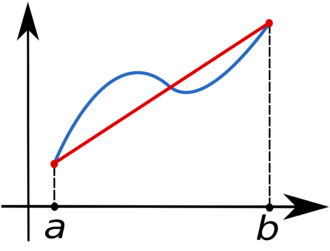
\includegraphics[scale=0.5]{trapez1.png}
\caption{The simplest form of the trapezoidal rule.}
\label{fig:simple_trapez}
\end{figure}
Figure \ref{fig:simple_trapez} has only one picture. For pictures appearing side by side see section \ref{subfigures}.

\subsection{Figures side by side}\label{subfigures}
This is how you put two pictures side by side. Note that each subfigure has its own caption, and the entire figure has a caption which gives a more general description of the figures. Figure \ref{fig:trapez1} is the same as figure \ref{fig:simple_trapez}. They both correspond to equation \eqref{eqn:trapez1}. Figure \ref{fig:trapez2} corresponds to equation \eqref{eqn:trapez2}. Figure \ref{fig:trapez} is a pictorial description of equations \eqref{eqn:trapez1}, and \eqref{eqn:trapez2}.
\begin{figure}
    \centering
    \begin{subfigure}[b]{0.4\textwidth}
        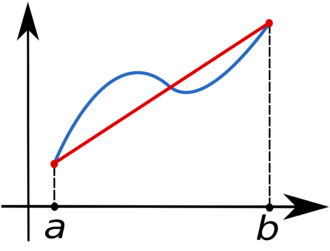
\includegraphics[width=\textwidth]{trapez1.png}
        \caption{Trapezoidal rule with a single strip.}
        \label{fig:trapez1}
    \end{subfigure}
    ~ %add desired spacing between images, e. g. ~, \quad, \qquad, \hfill etc. 
      %(or a blank line to force the subfigure onto a new line)
    \begin{subfigure}[b]{0.4\textwidth}
        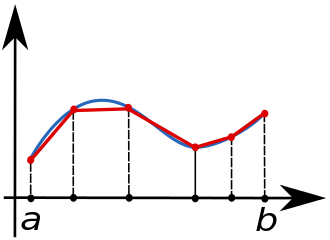
\includegraphics[width=\textwidth]{trapez2.png}
        \caption{Trapezoidal rule with $N$ equally spaced strips.}
        \label{fig:trapez2}
    \end{subfigure}
    \caption{Trapezoidal rules}\label{fig:trapez}
\end{figure}

%%%%%%%%%%%%%%%%%%%%%%%%%%%%%%%%%%%%%%%%%%%%%%%%%%%%%%%%%%%%%%%%%%%
\newpage
\section{Bibliography}
We shall only consider the simplest form of referencing. Later we shall look at the more general way of producing bibliography via bibtex. The format is basically given as follows:

\begin{verbatim}
\begin{thebibliography}{99}

  \bibitem{notes} John W. Dower {\em Readings compiled for History
  21.479.}  1991.

  \bibitem{impj}  The Japan Reader {\em Imperial Japan 1800-1945} 1973:
  Random House, N.Y.

  \bibitem{norman} E. H. Norman {\em Japan's emergence as a modern
  state} 1940: International Secretariat, Institute of Pacific
  Relations.

  \bibitem{fo} Bob Tadashi Wakabayashi {\em Anti-Foreignism and Western
  Learning in Early-Modern Japan} 1986: Harvard University Press.

\end{thebibliography}
\end{verbatim}

\subsection{Examples: How to cite}
To cite a reference, you use  $\setminus$cite$\{$key$\}$. For example: For a compiled reading history see \cite{notes}. To know more about Western learning in mordern Japan, we recommend \cite{fo, notes}. There is a comprehensive write up in \cite{norman} about the emergence of Japan as a modern state.

\newpage
\begin{thebibliography}{99}

  \bibitem{notes} John W. Dower {\em Readings compiled for History
  21.479.}  1991.
  
  \bibitem{norman} E. H. Norman {\em Japan's emergence as a modern
  state} 1940: International Secretariat, Institute of Pacific
  Relations.

  \bibitem{fo} Bob Tadashi Wakabayashi {\em Anti-Foreignism and Western Learning in Early-Modern Japan} 1986: Harvard University Press.
\end{thebibliography}

\end{document}